


\chapter{Terrain Assessment}
\label{cha:terain_assessment}
To make a successful coverage path planning, good information about what regions of the environment that has to be covered is a necessity. This chapter describes how traversable regions in a point cloud was found.

\section{Problem}
The problem that has to be solved is to distinguish which points in a given point cloud are accessible for the sweeping robot. In many applications all accessible points should be covered. We make following definitions for individual points (see figure \ref{fig:pointdefinitions}):
\begin{itemize}
    \item \textbf{Obstacle} - Point that can not be inside or in contact with the robot body  
    \item \textbf{Traversable} - Point that can be visited by the robot without collision with an obstacle
    \item \textbf{Coverable} - A point that could be covered by the range of the robot. After visiting every traversable point, all points that has been within the range of the robot are coverable.
    \item \textbf{Inaccessible} - Traversable and coverable points that are not accessible since there are no feasible path to reach them from the main coverable area. 
\end{itemize}

\begin{figure}
    \centering
    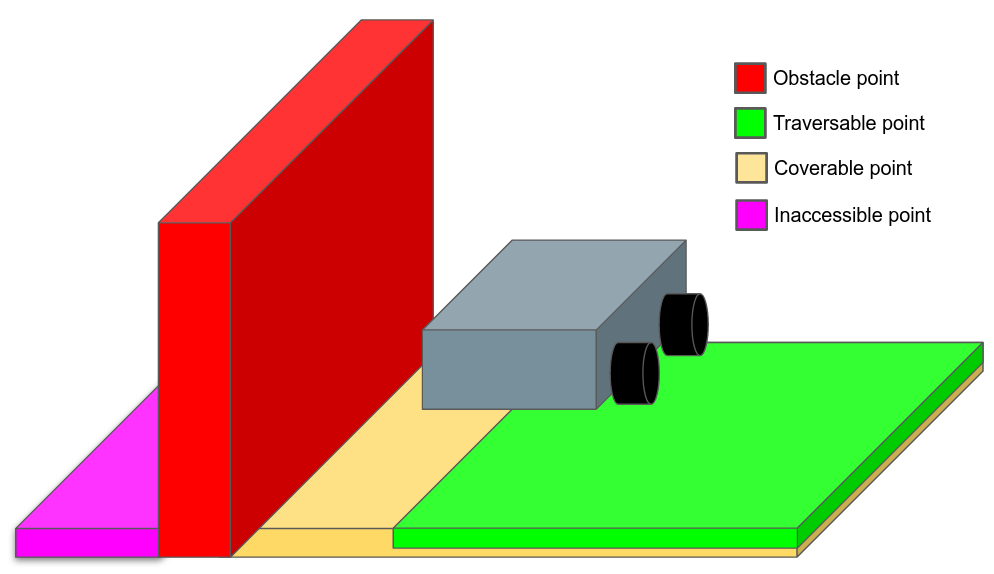
\includegraphics[width=0.7\textwidth]{figures/pointdefinitions.png}
    \caption{Point definitions.}
    \label{fig:pointdefinitions}
\end{figure}

For comuptational reasons, the point cloud of the environment can be arbitary discretized into floors and cells to avoid calculating traversability for every point. Every floor consists of a two dimensional cell grid, where every cell has an elevation height. The size of these cells has to be at maximum the size of the robot footprint area and could be smaller for a result with higher resolution. A cell can be:

\begin{itemize}
    \item \textbf{Invalid} - If the number of points in the cell is to low.
    \item \textbf{Ground} - If the elevation height of the cell is close to the lowest point of the floor.
    \item \textbf{Obstacle} - A cell with a wall or an obstacle that makes it unaccessible by the robot.
    \item \textbf{Inaccessible} - Cell that are not accessible since there are no feasible path to reach it from the main coverable area. 
    \item \textbf{Coverable} - A cell that could be covered by the robot. The criterias are described below.
    \item \textbf{Border} - An Obstacle or Invalid cell that has a Coverable cell as neighbour. 
\end{itemize}


Coverable points can only exist in coverable cells. Points in all other cells are classified as Obstacle. Only points that are close to the elevation height of the cell are classified as coverable, the rest are Obstacle points as well.

The criterias of a coverable cell is based on three parameters:
\begin{itemize}
    \item \textbf{Minimum floor height}, $h^{F}_{min}$  - the minimum height of free space in a cell. Free space is the space between the elevation height of the cell and the lowest point above it, see figure \ref{fig:freespace}
    \item \textbf{Maximum step height}, $h^{R}_{max}$ - the height difference between two points that the robot is able to get over without getting stuck, see figure \ref{fig:maxstepheight}
    \item \textbf{Minimum number of coverable points in cell}, $N^{cov}_{min}$ - tuned constant to exclude cells with insufficient information. The constant is representing a minimum amount of coverable points in the cell to make it count as valid.
\end{itemize}
The first two are robot specific, while the third is a hand tuned constant that depends on the density of the point cloud. 

\begin{figure}
    \centering
    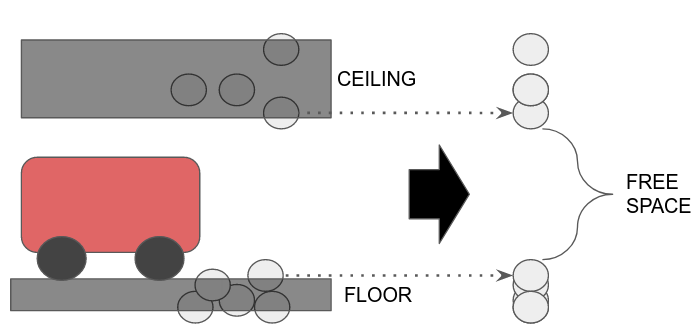
\includegraphics[width=0.7\textwidth]{figures/freespace.png}
    \caption{Definition of free space. It is detected by sorting the z-values of all points in the cell and find two following points with a height difference bigger than the robot height.}
    \label{fig:freespace}
\end{figure}

\begin{figure}
    \centering
    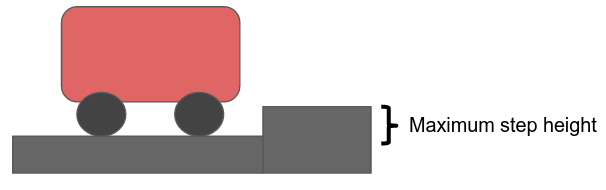
\includegraphics[width=0.7\textwidth]{figures/maxstepheight.png}
    \caption{Definition of the maximum step height. The biggest difference that the robot can go over without getting stuck}
    \label{fig:maxstepheight}
\end{figure}
 
The requirements for a coverable cell is following,
 \begin{itemize}
     \item The height difference between the cell and at least one of it's neighbors has to be lower than the maximum robot step $h^{R}_{max}$.
     \item The minimum floor height $h^{F}_{min}$ has to be bigger than the height of the robot $h_R$.
     \item Amount of coverable points in the cell has to be bigger than the minimum number of coverable points in cell constant $N^{cov}_{min}$
     \item Should be accessible from other coverable cells.
 \end{itemize}

\section{Method}
The method that was used to find all traversable and coverable points in a point cloud can be divided into four parts. These parts are described below. The 

\subsection{Floor Segmentation}
The first step was to divide the point cloud into different floors. Following steps, proposed in \cite{terrainassessment}, were made:
\begin{enumerate}
    \item The point cloud was divided into thin boxes with thickness $\Delta h_{L}$ laying upon each other.
    \item The amount of points in every box were counted.
    \item A histogram was made and the local maximas were identified.
    \item If the number of points in the local maxima was bigger than a threshold $N^{F}_{min}$, which was an arbitrarily hand tuned parameter, a potential ground height of a floor had been identified.
    \item The potential ground heights were examined to detect ceilings of rooms by requiring height difference of at least $h^{F}_{min}$.  
    \item When the ground height of every floor was known, the original point cloud was cut at these heights into segments. The result is one point cloud for each floor.
\end{enumerate}

\subsection{Cell Segmentation}
Next step was to make a discrete elevation model (DEM) of each floor, $E_i$. The point cloud of the floors was transformed into a 2D grid with cells, where every cell has an elevation height. It was assumed that every valid cell had only one elevation, $e_c$. The method to find the elevation height was proposed in \cite{terrainassessment}.

Firstly, the point cloud was simply projected on a 2D plane and divided into square cells, $M$. Secondly, the elevation for every cell was found and invalid cells were detected. It was done using Algorithm \ref{alg:elevation}. The idea of the algorithm was to sort the $z$-values for all points in a cell and then find two following points with a height difference that was bigger than the robot height $h_R$. The elevation height of the cell in the DEM was set to the height of the lowest point.

\begin{algorithm}[H]
\SetAlgoLined
\KwData{$M$, 2D-grid of environment, \\$P$, point cloud\\ $z^F$, floor ground height\\ Minimum number of coverable points in cell $N^{cov}_{min}$\\ Robot height $h_R$ \\Maximum step height $h^R_{max}$}
\KwResult{$E$, DEM of the environment}
 \For{\textup{cell $c \in  M$}}{
    $P_c$ = \textup{points in $P$ inside cell $c$}\\
    $Z_c$ = \textup{z-values of } $P_c$\\
    \For{$z_i$ \textup{in sorted} $Z_c$}{
        \If{|$z_{i-1}$ - $z_{i}$| > $h_R$}{
            \textup{\textbf{break}}\\
        }
    }
    $e_c$ = $z_{i-1}$ \\
    $P_{c, cov}$ = \textup{Points in $P_c$ with a $z$ closer than $h^R_{max}$ from $e_c$ } \\
    \eIf{\textup{Number of points in $P_{c, cov}$ > $N^{cov}_{min}$}}{
        \textup{Add a valid cell $c$ with $e_c$ as elevation height and $P_{c, cov}$ as coverable points to $E$} \\
    }{
        \textup{Add $Invalid$ cell $c$ to $E$} \\
    }
  }
 \caption{Find elevation for each cell and detect invalid cells}
 \label{alg:elevation}
\end{algorithm}

\subsection{Cell Classification}
After finding the elevation height of the cells, the heights were used to classify the accessibility of the cells for the robot. Some of the cells were already classified as $Invalid$ in the previous step. The classification algorithm is described in Algorithm \ref{alg:classification_coverable}. It is based on the idea of doing a breadth first search starting from a ground cell which was presented in \cite{terrainassessment}. 

First, all ground cells, cells with the same height as the lowest z of the floor, $z^F$ were inserted into a set of ground cells $E_{ground}$. All these cells are potential starting points for a cluster of connected coverable cells, an \emph{island}. These islands were built using a breadth first search on the DEM of the environment. When all islands had been detected, the biggest island, consisting the biggest amount of cells was chosen as the main coverable area, $E_{cov}$. All cells in $E_{cov}$ were classified as $Coverable$. Cells in other islands were classified as $Inaccessible$. Cells that were neither $Invalid$, $Coverable$ or $Inaccessible$ were classified as $Obstacle$. 

For later calculations of traversable points a set of border cells, $E_{border}$ had to be generated. This was done by looking for uncoverable neighbours of every cell of the main covarble area, see details in Algorithm \ref{alg:classification_border}. 

\begin{algorithm}[H]
\SetAlgoLined
\KwData{$z^F$, floor ground height \\ $E$, DEM of the environment}
\KwResult{$E_{cov}$, Coverable cells}
 $E_{ground}$ = \textup{cells in $E$ with elevation close to $z^F$} \\
 $I = \emptyset$ \\
\While{$E_{ground} \neq \emptyset$ }{
    \textup{$c_{start} \leftarrow$ arbitrary cell in $E_{ground}$}\\
    $E_{visited} = \{c_{start}\}$ \\
    $Q_{cov} = \{c_{start}\}$ \\
    \While{$Q_{cov} \neq \emptyset$}{
        $c_{curr} \leftarrow Q_{cov}.\texttt{pop()}$ \\
        \For{\textup{neighbour} $c_n$ \textup{of} $c_{curr}$}{
            \If{\textup{$c_n$ is not accessible from $c_{curr}$}}{
                \textup{\textbf{continue\\}}}
            \If{\textup{$c_n$ is in $E_{visited}$}}{
                \textup{\textbf{continue\\}}}
            \If{\textup{$c_n$ is in $E_{ground}$}}{
                $E_{ground}$ = $E_{ground}$ / $c_n$}
            $E_{visited}$ = $E_{visited} \cup c_n$ \\
            $Q_{cov}.\texttt{push}(c_n)$
        } \\
    }
    $I = I \cup E_{visited}$ \\
}
$E_{cov}$ = \textup{the set with biggest amount of cells in $I$} \\
\textup{\textbf{return} $E_{cov}$} 
 \caption{Detect the main coverable area}
 \label{alg:classification_coverable}
\end{algorithm}

\begin{algorithm}[H]
\SetAlgoLined
\KwData{$E_{cov}$, Coverable cells, $E$, DEM of the environment}
\KwResult{$E_{border}$ Border cells}
$E_{border}$ = \emptyset \\
\For{\textup{cell $c$ in $E_{cov}$}}{
    \For{\textup{neighbour $c_n$ of $c$ in $E$}}{
        \If{\textup{$c_n$ is not in $E_{cov}$}}{
            \textup{$E_{border} = E_{border} \cup c$} \\
        }
    }
}
\textup{\textbf{return} $E_{border}$ } 
 \caption{Detect all Border cells of the main coverable area}
 \label{alg:classification_border}
\end{algorithm}

\subsection{Point Classification}
The last step in the terrain assessment is to classify the points into $Traversable, Coverable$ and $Obstacle/Inaccessible$. The purpose is to stop the path planning from making waypoints that are close to obstacles, where there is a risk of collision. 

First, all coverable points for every cell in the main coverable area $E_{cov}$ was extracted as a potentially coverable point cloud $P_{p, cov}$. Then, a point was created for every border cell in $E_{border}$ and put into a border point point cloud $P_{border}$. The ($x,y$)-position of the created points were set to the center position of the border cell. The $z$ value was set to the elevation height of the neighbouring coverable cell in $E_{cov}$. 

A point was classified as $Traversable$ if the distance to the closest border point was bigger than

$$
d_{collision} = \frac{1}{\sqrt{2}} s_c + 0.5  b_R
$$
where $s_c$ is the size of the cells in the cell grid and $b_R$ is the breadth of the robot. See motivation and explanation in Figure \ref{fig:dcollision}.

\begin{figure}
    \centering
    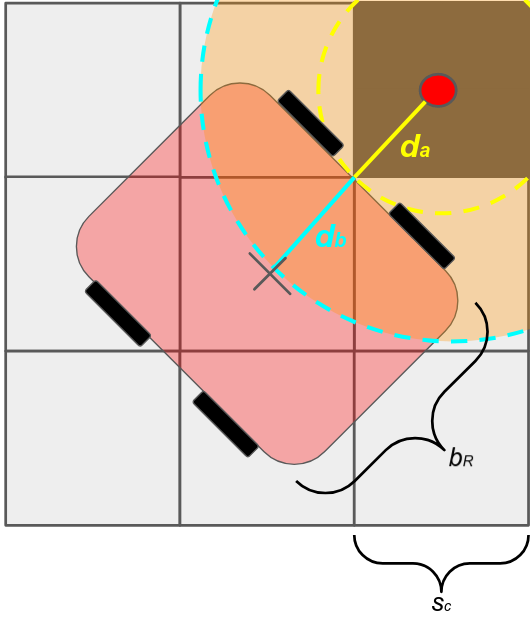
\includegraphics[width=0.5\textwidth]{figures/dcollision.png}
    \caption{Illustration of the distance $d_{collision} = d_a + d_b$, where $d_a =  \frac{1}{\sqrt{2}} s_c$ and $d_b = 0.5 b_R$. The red point is a border point. Yellow area is untraversable due to risk of collision. $s_c$ is the size of the cells and $b_R$ is the breadth of the robot}
    \label{fig:dcollision}
\end{figure}

The idea was to first assume that every coverable point was $Traversable$, and then go through every border point and set points nearby as untraversable. Thereafter, the algorithm detects all inaccessible points by finding coverable points that are not within the robot range from a traversable point. It is assumed that the robot covers all points within a radius $r_R$ from the position of the robot. The algorithm is described in detail in algorithm \ref{alg:traversability} and illustrated in figure \ref{fig:pointclassification}.

\begin{figure}
    \centering
    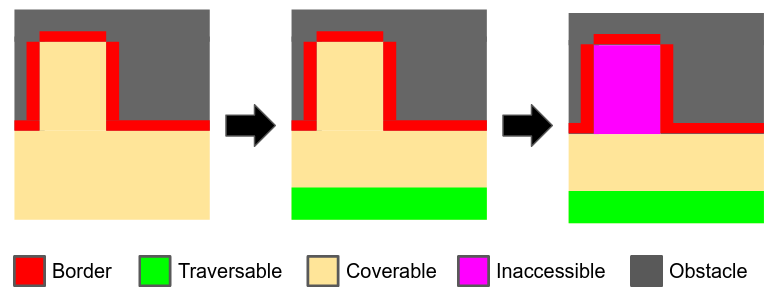
\includegraphics[width=0.9\textwidth]{figures/pointclassification.png}
    \caption{Illustration of the point classification algorithm. First, border points and potential coverable points are identified. Secondly, coverable points that are not close to border points are classified as traversable. Thirdly, only points that are reachable from the traversable points are classified as coverable, the rest are inaccessible.}
    \label{fig:pointclassification}
\end{figure}

\begin{algorithm}[H]
\SetAlgoLined
\KwData{Potentially coverable point cloud $P_{p, cov}$, point cloud with border points, $P_{border}$, distance from a border point to robot position with no risk of collision, $d_{collision}$. Radius range of robot $r_R$}
\KwResult{Coverable point cloud, $P_{cov}$, Traversable point cloud, $P_{trav}$}
$P_{trav}$ = $P_{p, cov}$ \\
\For{\textup{point $p$ in $P_{border}$}}{
     \textup{$P_{collision}$ = points in $P_{trav}$ closer than $d_{collision}$ from $p$} \\
     $P_{trav}$ = $P_{trav}$ / $P_{collision}$ \\
}
$Q_{cov}$ = $P_{p, cov}$ / $P_{trav}$ \\
$P_{cov}$ = $P_{p, cov}$ \\
\While{\textup{$Q_{cov} \neq \emptyset$}}{
    $p_{cov}$ \leftarrow $Q_{cov}.\texttt{pop()}$ \\
    \If{\textup{ distance from $p_{cov}$ to the closest point in $P_{trav}$ is bigger than $r_R$ }}{
        $P_{cov}$ = $P_{cov}$ / $p_{cov}$
    }
}

\textup{\textbf{return} $P_{cov}$, $P_{trav}$ } 
 \caption{Find traversable positions for the robot and all coverable points.}
 \label{alg:traversability}
\end{algorithm}

\section{Result}
Two floors were detected in the point cloud. The histogram in figure \ref{fig:floorsegmentation} shows the number of points for different heights. By looking at the histogram a tuned threshold value $N^F_{min}$, represented as the orange line in the figure, was chosen to leave the three highest peaks as potential ground heights. Since the peak in the middle does not fulfill the requirement of having $h^F_{min}$ meters free until next peak, the floor segmentation algorithm classified it as ceiling. Finally, the other two peaks defined the heights of the floor ground and the point cloud could be divided. 

Values and explanation of all parameters used are presented in Table \ref{tab:TAparameters}. The result of the terrain assessment is shown in figure \ref{fig:terrainassessment} and tables \ref{tab:cellclasses} and \ref{tab:pointclasses}.  



\begin{table}[]
    \centering
    \caption{Parameters used in Terrain Assessment. Values of \emph{Real data} parameters are based on data from the real world provided by the developers of the robot. Values of \emph{Resolution} parameters are minimised to give a good resolution while keeping the computational time on a reasonable level. \emph{Hand tuned based on point cloud} parameters are hand tuned by looking at the generated classification results and make them plausible with the given point cloud. \emph{Hand tuned based on histogram} is based on Figure \ref{fig:floorsegmentation}}.
    \begin{tabular}{|c|c|c|c|}
        \hline 
        \textbf{Parameter} & \textbf{Value} & \textbf{Explanation} & \textbf{Based on} \\
        \hline 
        $b_R$ & 0.75 m & Breadth of robot & Real data \\
        $h_R$ & 1 m & Height of robot & Real data \\
        $h^R_{max}$ & 0.1875 m & Max. step height of robot & Hand tuned b.o. point cloud  \\
        $s_c$ & 0.5 m & Cell size. Length of side. & Resolution  \\
        $\Delta h_L$ & 0.1 m & Thickness of each layer & Resolution  \\
        $h^F_{min}$ & 2 m & Min. height of a floor & Real data  \\
        $N^{cov}_{min}$ & 25 & Min. coverable points in cell & Hand tuned b.o. point cloud \\
        $N^{F}_{min}$ & $10^5$ & Min. points in ground layer & Hand tuned b.o. histogram \\
        \hline 
    \end{tabular}
    
    \label{tab:TAparameters}
\end{table}


\begin{figure}
    \centering
    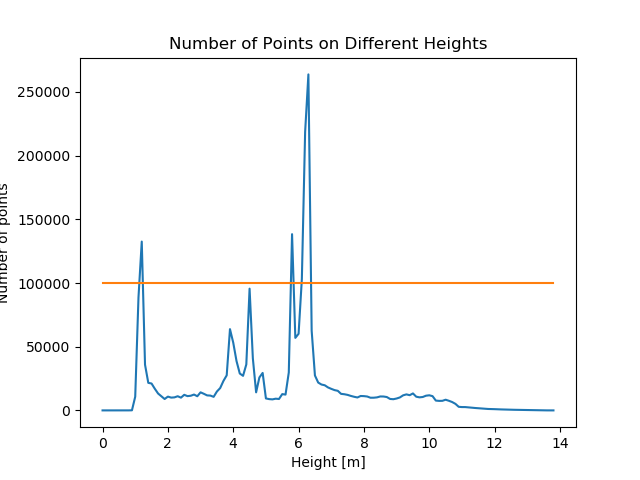
\includegraphics[width=0.9\textwidth]{figures/floorsegmentation.png}
    \caption{The histogram used for floor segmentation. Two major peaks at the height of around 1 and 6.5 meter can be identified. They represent the height of the ground of the two floors. The other peaks are obstacles and ceiling. The orange line represents the hand tuned \emph{Minimum number of coverable points in cell} parameter. By neglecting all peaks under this line it leaves only three peaks to possibly represent the height of a ground floor. The peak at 6 meter is then excluded, since it is less than 2 meter distance until next peak, which means that it is probably the points of the ceiling of the lower floor.}
    \label{fig:floorsegmentation}
\end{figure}



\begin{figure}
\centering
    \begin{subfigure}{.49\textwidth}
    \centering
    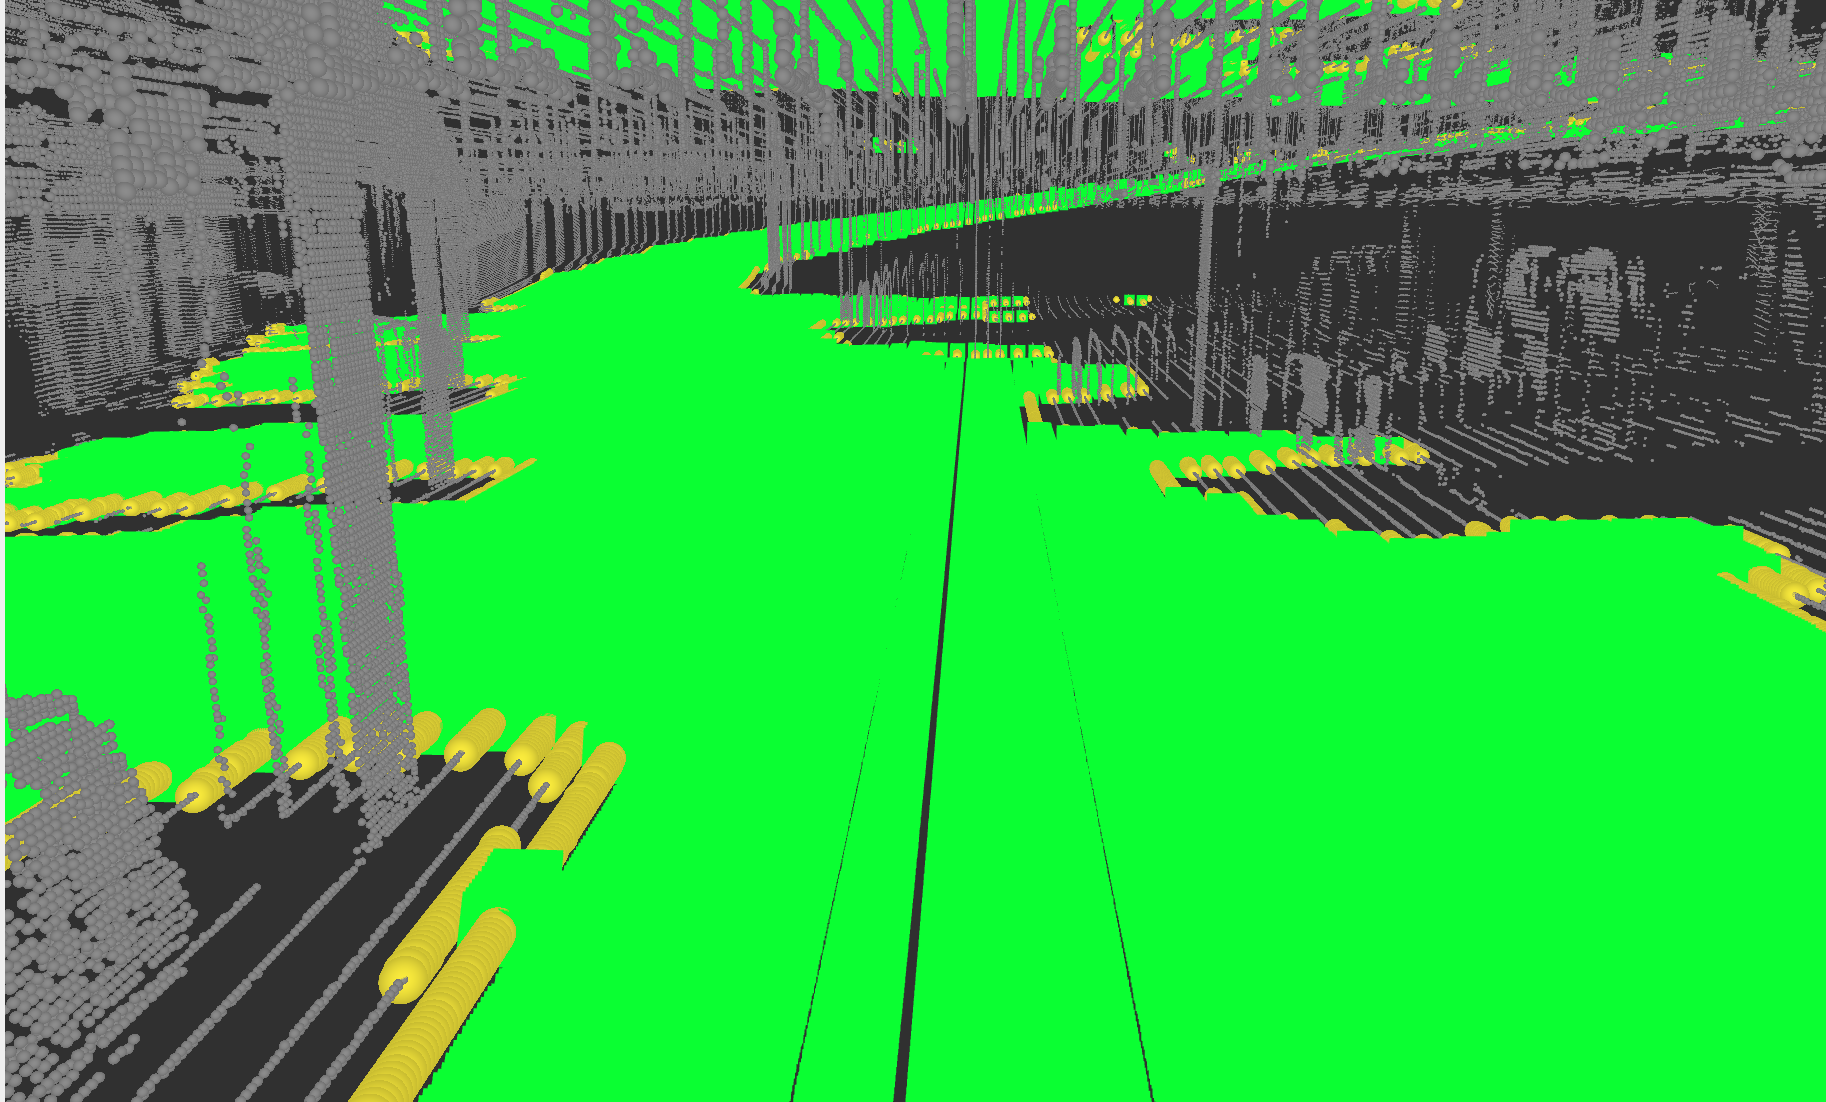
\includegraphics[width=\textwidth]{figures/terrainassessmentresult-floor1.png}
    \caption{Floor 1}
    \end{subfigure}
    \begin{subfigure}{.49\textwidth}
    \centering
    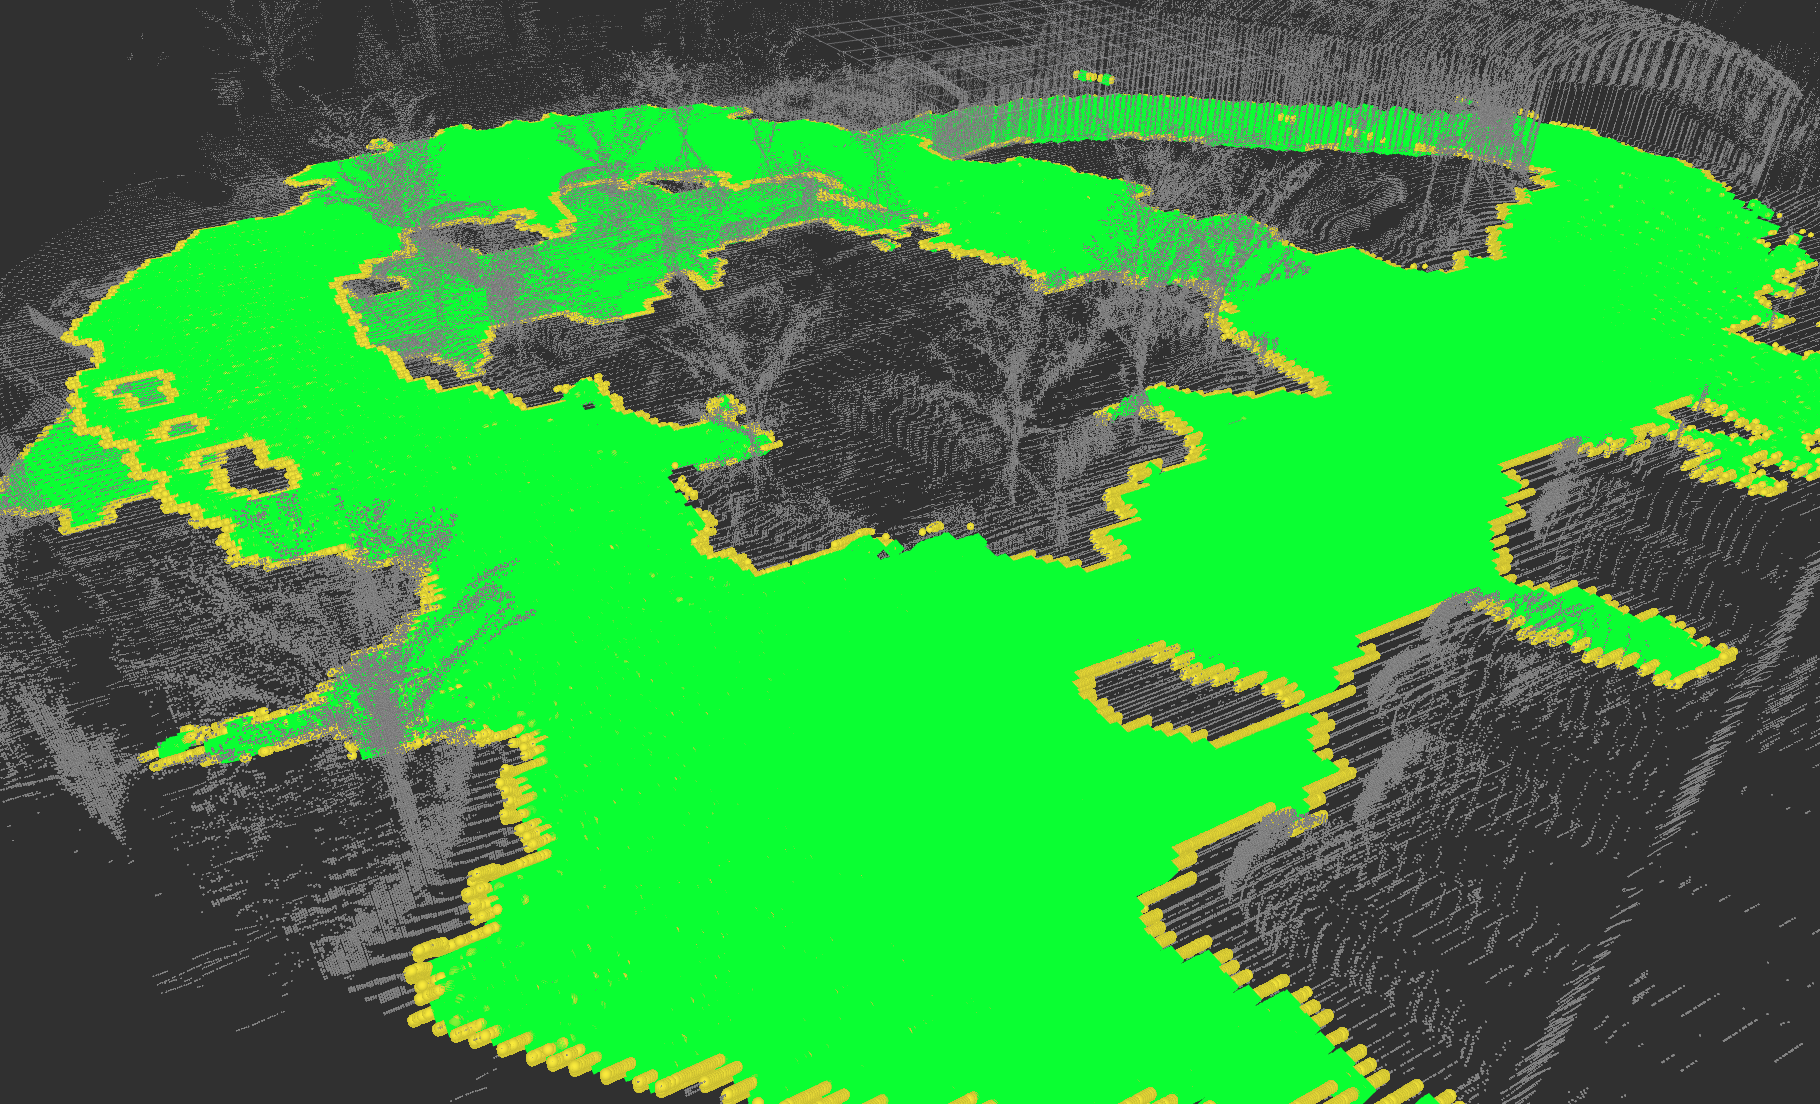
\includegraphics[width=\textwidth]{figures/terrainassessment-floor2'.png}
    \caption{Floor 2}
    
    \end{subfigure}
    
    \caption{Result of Terrain Assessment. Green points represents traversable areas, yellow are only coverable and grey are points that are obstacle and inaccessible points}
    \label{fig:terrainassessment}
\end{figure}

\begin{table}[]
\caption{Result Cell classification of the Terrain Assessment. COVERABLE area can possibly be covered by the robot. OBSTACLE area that has an elevation height that makes it inacessible. INACCESSIBLE are the area that could be covered, but is not connected to the main coverage area. INVALID area with cells that does not have enough information to be evaluated. TOTAL is the total area of the floor, including areas with no points. }

\begin{center}
\begin{tabular}{ |c|c|c|c|c|c| } 
\hline
Floor & COVERABLE & OBSTACLE & INACCESSIBLE & INVALID & TOTAL \\ 
 \# & $[m^2]$ & $[m^2]$  & $[m^2]$  & $[m^2]$  & $[m^2]$  \\ 
\hline
1 & 636 & 150 & 1 & 2433 & 3220 \\
2 & 1052 & 245 & 48 & 2225 & 3570\\
\hline

\end{tabular}
\end{center}
\label{tab:cellclasses}
\end{table}

\begin{table}[]
\caption{Result of Point Classification of Terrain Assessment. TRAVERSABLE points are positions that can be visited by the robot. If the robot would visit all these points all COVERABLE points would be covered. INACCESSIBLE are the points that could be covered, but is to far away from a TRAVERSABLE point. OBSTACLE points are not allowed to be within the range of the robot. TOTAL is the total number of points in the point cloud}
\begin{center}
\begin{tabular}{ |c|c|c|c|c| } 
\hline
COVERABLE & TRAVERSABLE & INACCESSIBLE & OBSTACLE & TOTAL \\ 
 \# & \# & \#  & \#  & \#  \\ 
\hline
1 140 545 (43\%) & 1 061 050 (40\%) & 52 311 (2\%) & 1 433 282 (55\%) & 2 626 138  \\
\hline

\end{tabular}
\end{center}
\label{tab:pointclasses}
\end{table}

\section{Discussion}
As shown in figure \ref{fig:terrainassessment} the results of the terrain assessment were quite reasonable. Points that were classified as traversable were on a distance from obstacle points with coverable points in between, similar to the illustration in figure \ref{fig:pointdefinitions}. 

A fault of this process is that it only makes sure that all coverable cells are connected in a main coverable area. The point classification does not ensure that all traversable points are connected. Therefore, a few small clusters of traversable points with connected coverable points are in fact inaccessible. 

The algorithm did also struggled with classifying some parts of the wall of the ramp. The floor segmentation divided the environment into two floors and classified the cells separately without taking the classification of the other floor into account. For a wall of a ramp that ranges over multiple floors this became a problem. The classification of the first floor classified wall points at the floor splitting height as coverable. Most of these points were later classified as inaccessible by the point classification, but it still caused some unexpected classifications of points on the ramp close to the wall, see figure \ref{fig:faulty_terrain_assessment}.

\begin{figure}
    \centering
    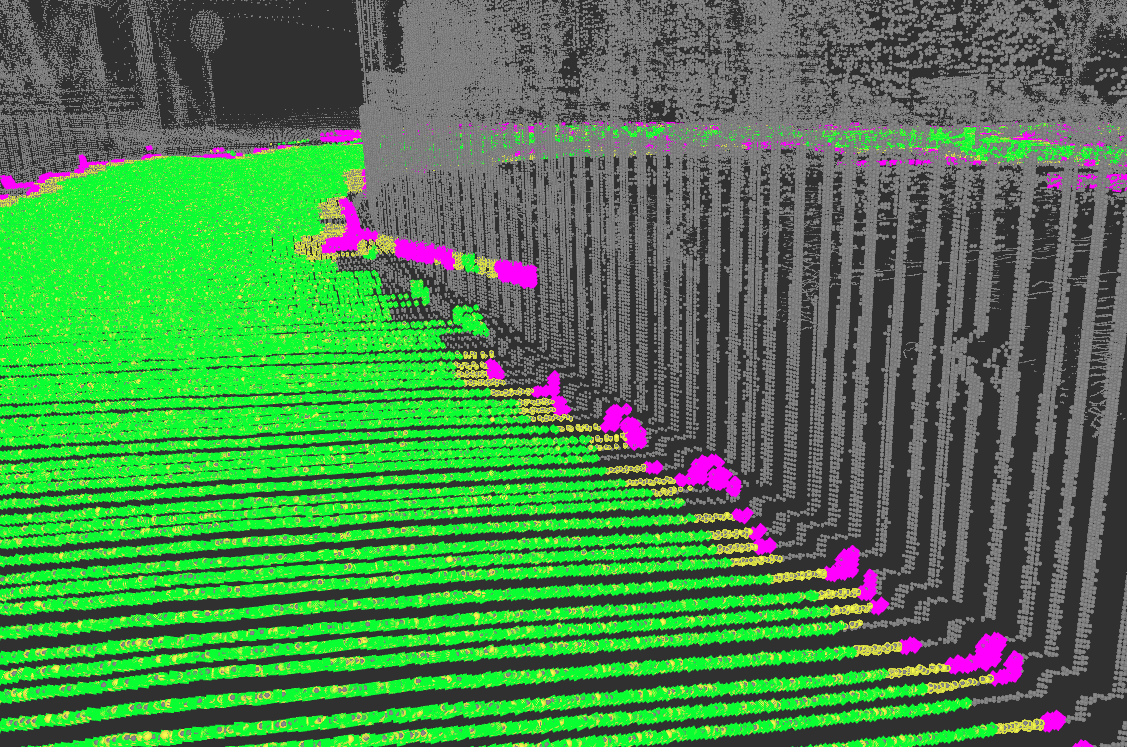
\includegraphics[width=0.9\textwidth]{figures/faulty_terrain_assessment.png}
    \caption{Part of the wall of the ramp where the terrain assessment did some unexpected classification due to faults in the algorithm. Green points are traversalbe, yellow points are coverable and purple points are inaccessible.}
    \label{fig:faulty_terrain_assessment}
\end{figure}


\section{3D Perspective (Will probably be removed)}
A few calculations were done to evaluate the need of an algorithm that takes the height dimension into consideration. This was made based on the method proposed in \cite{HAMEED201636}. The given poinctcloud has an inclined passage area, that connects the two floors. Since the rest of the traversable regions in the point cloud are flat, only this area is of interest in this section.

A simple approach to make a path that covers all cells would be to represent the cells as a 2D-grid and make a side-to-side path in a specific direction. A way to see how much the inclination affects the coverage efficiency of such path is to do the following:
\begin{enumerate}
    \item A cylinder were created for every traversable cell. It was rotated in a way that it's flat surfaces pointed in a given direction. This direction represented the driving direction of the robot, which is the same for every cylinder since the path goes from side to side all the way. The radius of these cylinders was the range of the robot, which was set to the same as the cell width. The length of the cylinder was set to the cell width as well to cover the cell, See figure \ref{fig:cylinders}.
    \item The amount of ground points that was inside the cylinder, $n_c$, and the total amount of ground points $n$ was counted. 
    \item Coverage efficiency, was given by \begin{equation}
        C_{eff} =\frac{n_c}{n} 
    \end{equation}
\end{enumerate}  

\begin{figure}
    \centering
    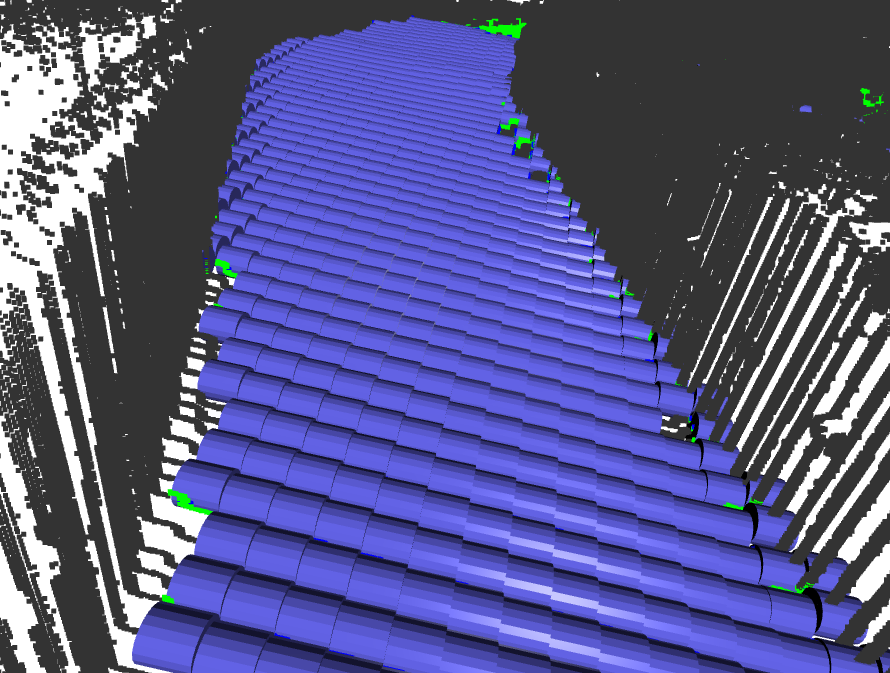
\includegraphics[width=\textwidth]{figures/tunnelskippedareascylinder.png}
    \caption{Cylinders were placed on every traversable cell to see how much the inclination affected the coverage efficiency of a simple 2D grid representation}
    \label{fig:cylinders}
\end{figure}

$C_{eff}$ for this point cloud was 71.6\%. The skipped areas are shown in figure \ref{fig:skippedareas}. Figure \ref{fig:cylinderzoom} shows a place where points were not covered by the cylinder because of the inclination. 

\begin{figure}
    \centering
    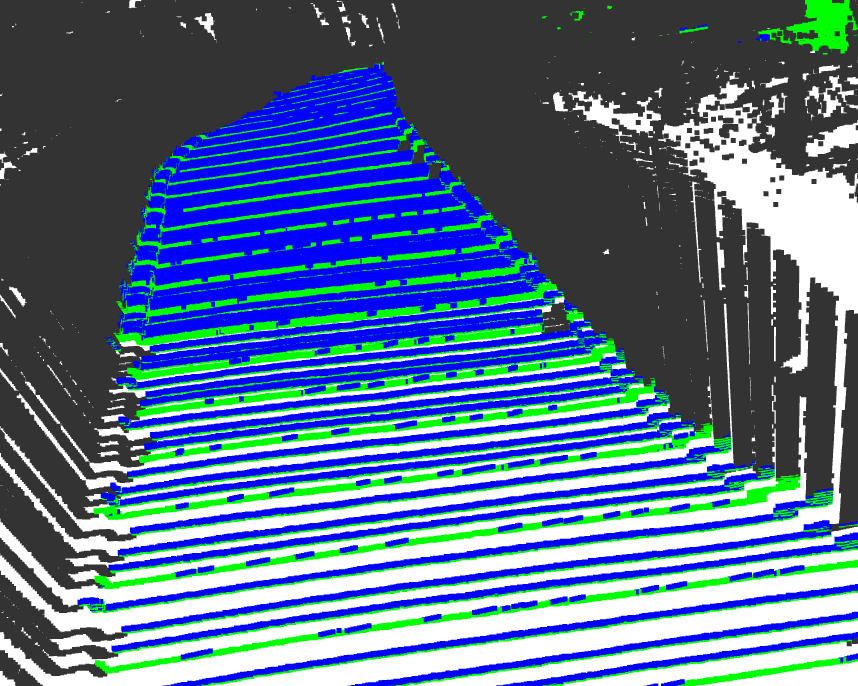
\includegraphics[width=\textwidth]{figures/tunnelskippedpoints.png}
    \caption{Covered points in blue and missed points in green. 71.6\% of the points were covered.}
    \label{fig:skippedareas}
\end{figure}

\begin{figure}
    \centering
    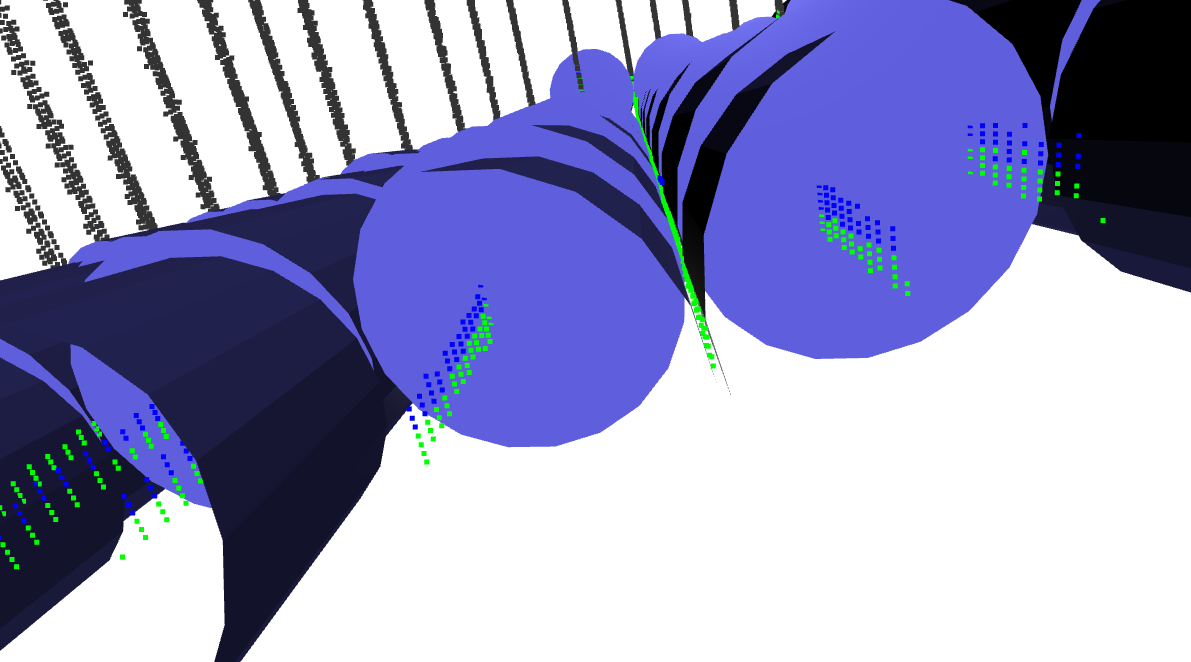
\includegraphics[width=\textwidth]{figures/tunnelskippedinzoom.png}
    \caption{A situation where a simple approach would not cover some points. The inclination is big enough to affect the range of the sweeping robot.}
    \label{fig:cylinderzoom}
\end{figure}

A coverage efficiency of 71.6\% is desirable to improve, however there are a few observations that should be considered. Firstly, the chosen direction of the cylinders was probably the worst case scenario. When the direction was changed to make the robot go up and down the ramp, instead of side-to-side, the efficiency went up to 95.0\%, see Figure \ref{fig:cylinderupdown}. Secondly, there might be some errors in the calculations due to approximations or misleading coincidences. The given point cloud consists of lines of points, which in the worst case appears right between the cylinders, which is the case in figure \ref{fig:cylinderzoom}. This makes it more sensitive to small inclinations, which lowers the coverage efficiency significantly. By extending the radius or moving the paths sideways only a few centimeters, the coverage efficiency could be improved by almost 20\%. This shows that the precision of this method is not reliable for this point cloud. However, it could still be used to motivate that a coverage path planning algorithm should take height differences into consideration when planning a path in environments with inclination.


\begin{figure}
\centering
    \begin{subfigure}{.49\textwidth}
    \centering
    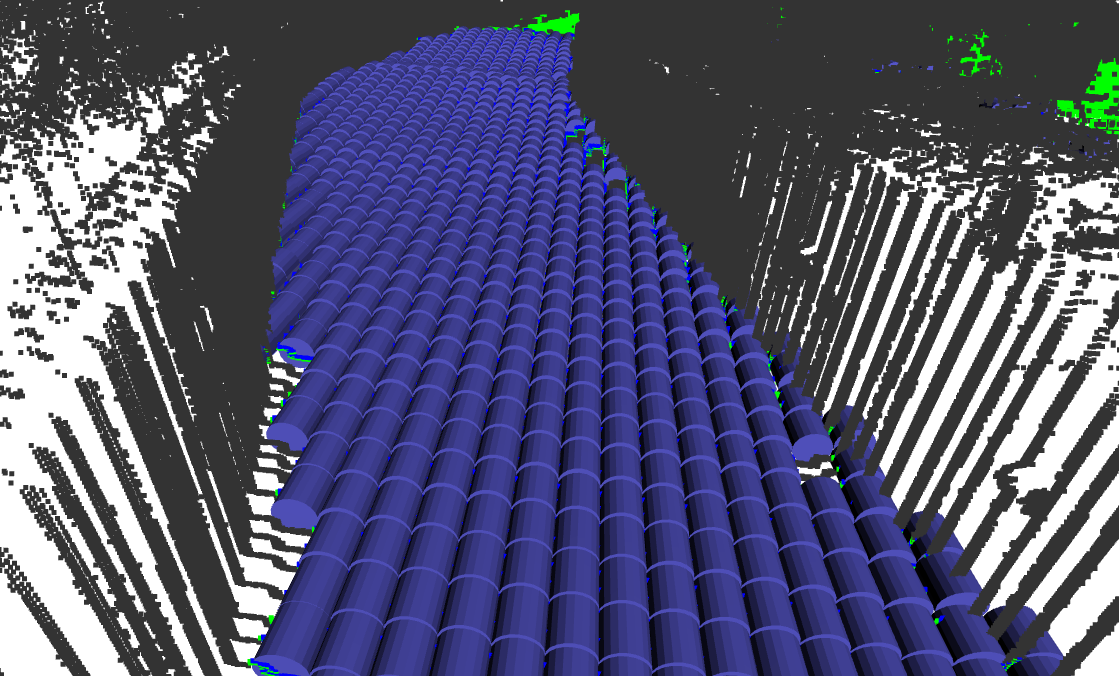
\includegraphics[width=\textwidth]{figures/cylinderupdown.png}
    \caption{With cylinders}
    \end{subfigure}
    \begin{subfigure}{.49\textwidth}
    \centering
    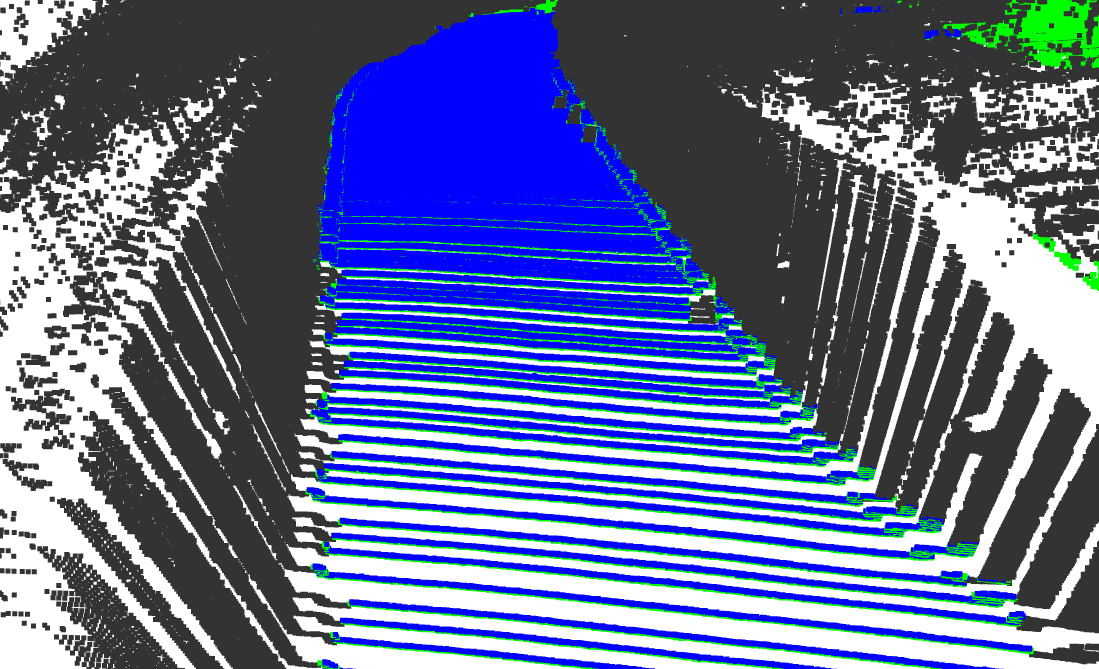
\includegraphics[width=\textwidth]{figures/nocylinderupanddown.png}
    \caption{Without cylinders}
    
    \end{subfigure}
    
    \caption{If the direction is changed to make the robot go up and down the ramp, the coverage efficiency improves significantly.}
    \label{fig:cylinderupdown}
\end{figure}